\chapter{Theoretical Foundations and Methods}\label{sec:theoryandmethods}

CHECK FOOTNOTE NUMBERS IN WHOLE DOCUMENT!
\section{Quantum Bits}
\label{subsec:qubits}

INTRODUCE CONCEPT OF T1 and T2!

\subsection{Single Qubit Systems}
\label{subsubsec:qubits}
%Classical computers manipulate bits and the quantum equivalent is called a quantum bit, often abbreviated as qubit.
Classical computers manipulate bits, whereas quantum computer's most fundamental unit is called a quantum bit, often abbreviated as qubit. Bits as well as qubits are binary entities, meaning they can only take the values 0 and 1.

A good example for a physical implementation of a qubit is the single electron of a hydrogen atom sketched in Fig.~\ref{img:qubitatom}. Usually, the electron is found in its ground state which one can define as the \0 state of the qubit. Using a laser pulse the electron can be excited into the next highest valence shell which one can define as the \1 state of the qubit. After some time $t$ the electron will decohere to its ground state (\0) which is called the longitudinal coherence or amplitude damping time and is an important parameter for measuring qubit lifetimes.

\begin{figure}[!ht]
       \centering
       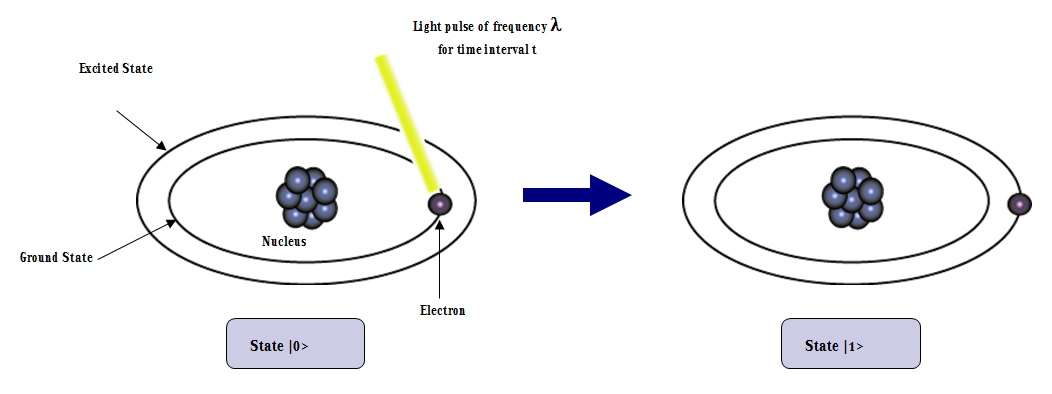
\includegraphics[width=0.9\textwidth]{img/qubitimplementation.jpeg}
       \caption{\label{fig:qubitatom} A simple example of a physical qubit using the electron of a hydrogen atom}
\end{figure}

\footnotetext[1]{Reprinted from RF Wireless World, n.d., Retrieved December 23, 2016, from \url{http://www.rfwireless-world.com/Terminology/Difference-between-Bit-and-Qubit.html}. Copyright 2012 by RF Wireless World. Reprinted with permission.}

A classical non-probabilistic bit can only be in one of the two possible states at once. In contrast, qubits obey the laws of quantum mechanics, which gives rise to the powerful property that - besides being a definite 0 or 1 - they can also be in a superposition of the two states. Mathematically this is expressed as a linear combination of the states 0 and 1:

\begin{equation}
\label{equ: simplequbit}
\ket{\psi} = \alpha \ket{0} + \beta \ket{1}
\end{equation}

where $\alpha$ and $\beta$ are complex coefficients ($\alpha, \beta \in \mathbb{C}$) and are often referred to as phase factors or amplitudes. \0 is the Dirac notation for the qubit being in state 0 and it represents a two-dimensional vector in a complex 2-D vector space (called Hilbert space $\mathcal{H}_{2}$). \0 and \1 are the computational basis states and they constitute an orthonormal basis of $\mathcal{H}_{2}$. For the sake of clarity, \0 and \1 can be thought of as the 2-D vectors shown below.
\begin{equation}
\label{equ: 0and1kets}
\ket{0} =  \colvec{1\\0} \quad \quad \ket{1} = \colvec{0\\1}
\end{equation}

Subbing these vectors into Equ.~\ref{equ: simplequbit} yields the vector representation of $\ket{\psi}$:
\begin{equation}
\label{equ: simplequbitvector}
\ket{\psi} = \alpha \colvec{1\\0} + \beta \colvec{0\\1} = \colvec{\alpha\\\beta}
\end{equation}

Another important qubit lifetime parameter is the transversal coherence or phase damping time. It is measured by preparing the equal superposition $\frac{\ket{0}+\ket{1}}{\sqrt{2}}$ and due to inavoidable interaction with the environment after some time $t$ the quantum behaviour will be lost and the state will either be a definite \0 or \1.

However, even though a qubit can be in a superposition of \0 and \1, when measured it will take the value \0 with a probability of
\begin{equation}
\label{equ:bornrule0}
Prob(\ket{0}) = {|\alpha|}^{2}
\end{equation}
and \1 with a probability of 
\begin{equation}
\label{equ:bornrule1}
Prob(\ket{1}) = {|\beta|}^{2}
\end{equation}

The fact that the probability of measuring a particular state is equal the absolute value squared of the respective amplitude is called Born rule (citation). Since the total probability of measuring any value has to be 1, the following normalization condition must be satisfied:
\begin{equation}
\label{equ: normalization}
{|\alpha|}^{2} + {|\beta|}^{2} =  1
\end{equation}
Therefore, a qubit is inherently probabilistic but when measured it collapses into a single classical bit (0 or 1). It follows that a measurement destroys information about the superposition of the qubit (the values of $\alpha$ and $\beta$). This constitutes one of the main difficulties when designing quantum algorithms since only limited information can be obtained about the final states of the qubits in the quantum computer.

Similar to logic gates in a classical computer, a QC manipulates qubit by means of quantum logic gates which will be introduced in detail in Section~\ref{subsec:quantumlogicgates}. Generally, an arbitrary quantum logic gate U acting on a single qubit state is a linear transformation given by a 2x2 matrix whose action on $\ket{\psi}$ is defined as:

\begin{equation}
\label{equ:unitarytransformation}
U \ket{\psi} = \begin{pmatrix}
 a & b \\ 
 c & d
 \end{pmatrix} \colvec{\alpha\\\beta} = \colvec{a*\alpha+b*\beta\\c*\alpha+d*\beta}
\end{equation}

Matrix $U$ must be unitary which means that a) its determinant is equal to unity and b) its Hermitian conjugate $U^\dagger$ must be equal to its inverse. These properties are expressed in Equ.~\ref{equ:unitarydef1} and ~\ref{equ:unitarydef2} below. All quantum logic gates must be unitary since this preserves the normalization of the qubit state it is acting on.

\begin{align}
\label{equ:unitarydef1}
a)& \mid det(U) \mid = 1 \\ 
\label{equ:unitarydef2}
b)& \quad UU^\dagger = U^\dagger U = \mathbb{1} = UU^{-1} = U^{-1}U
\end{align} 

Using spherical polar coordinates, a single qubit can be visualized on the so-called Bloch sphere by parameterising $\alpha$ and $\beta$ in Equ.~\ref{equ: simplequbit} as follows:

\begin{equation}
\label{equ: blochqubit}
\ket{q} = \cos\frac{\theta}{2} \ket{0} + e^{i \phi} \sin\frac{\theta}{2} \ket{1}
\end{equation}

The Bloch sphere has a radius of 1 and is therefore a unit sphere. The \0 qubit state is defined to lie along the positive z-axis ($\hat{z}$) and the \1 state is defined to lie along the negative z-axis ($-\hat{z}$) as labelled in Fig.~\ref{fig:blochsphere}. At this point, it is important to note that these two states are mutually orthogonal in $\mathcal{H}_{2}$ even though they are not orthogonal on the Bloch sphere. 

Qubit states on the Bloch equator such as the $\hat{x}$ and $\hat{y}$ coordinate axes represent equal superpositions where \0 and \1 both have measurement probabilities equal to $0.5$. The $\hat{x}$-axis for example represents the equal superposition $\ket{q} = \frac{1}{\sqrt{2}} \ket{0} + \frac{1}{\sqrt{2}} \ket{1}$. As illustrated in Fig.~\ref{fig:blochsphere} any arbitrary 2-D qubit state $\ket{\psi}$ can be decomposed into the polar angles $\theta$ and $\phi$ and visualized as a vector on the Bloch sphere. Such an object is called the Bloch vector of the qubit state $\ket{\psi}$. The Bloch sphere will be the main visualization tool for qubit manipulations in this thesis.

\begin{figure}[!ht]
       \centering
       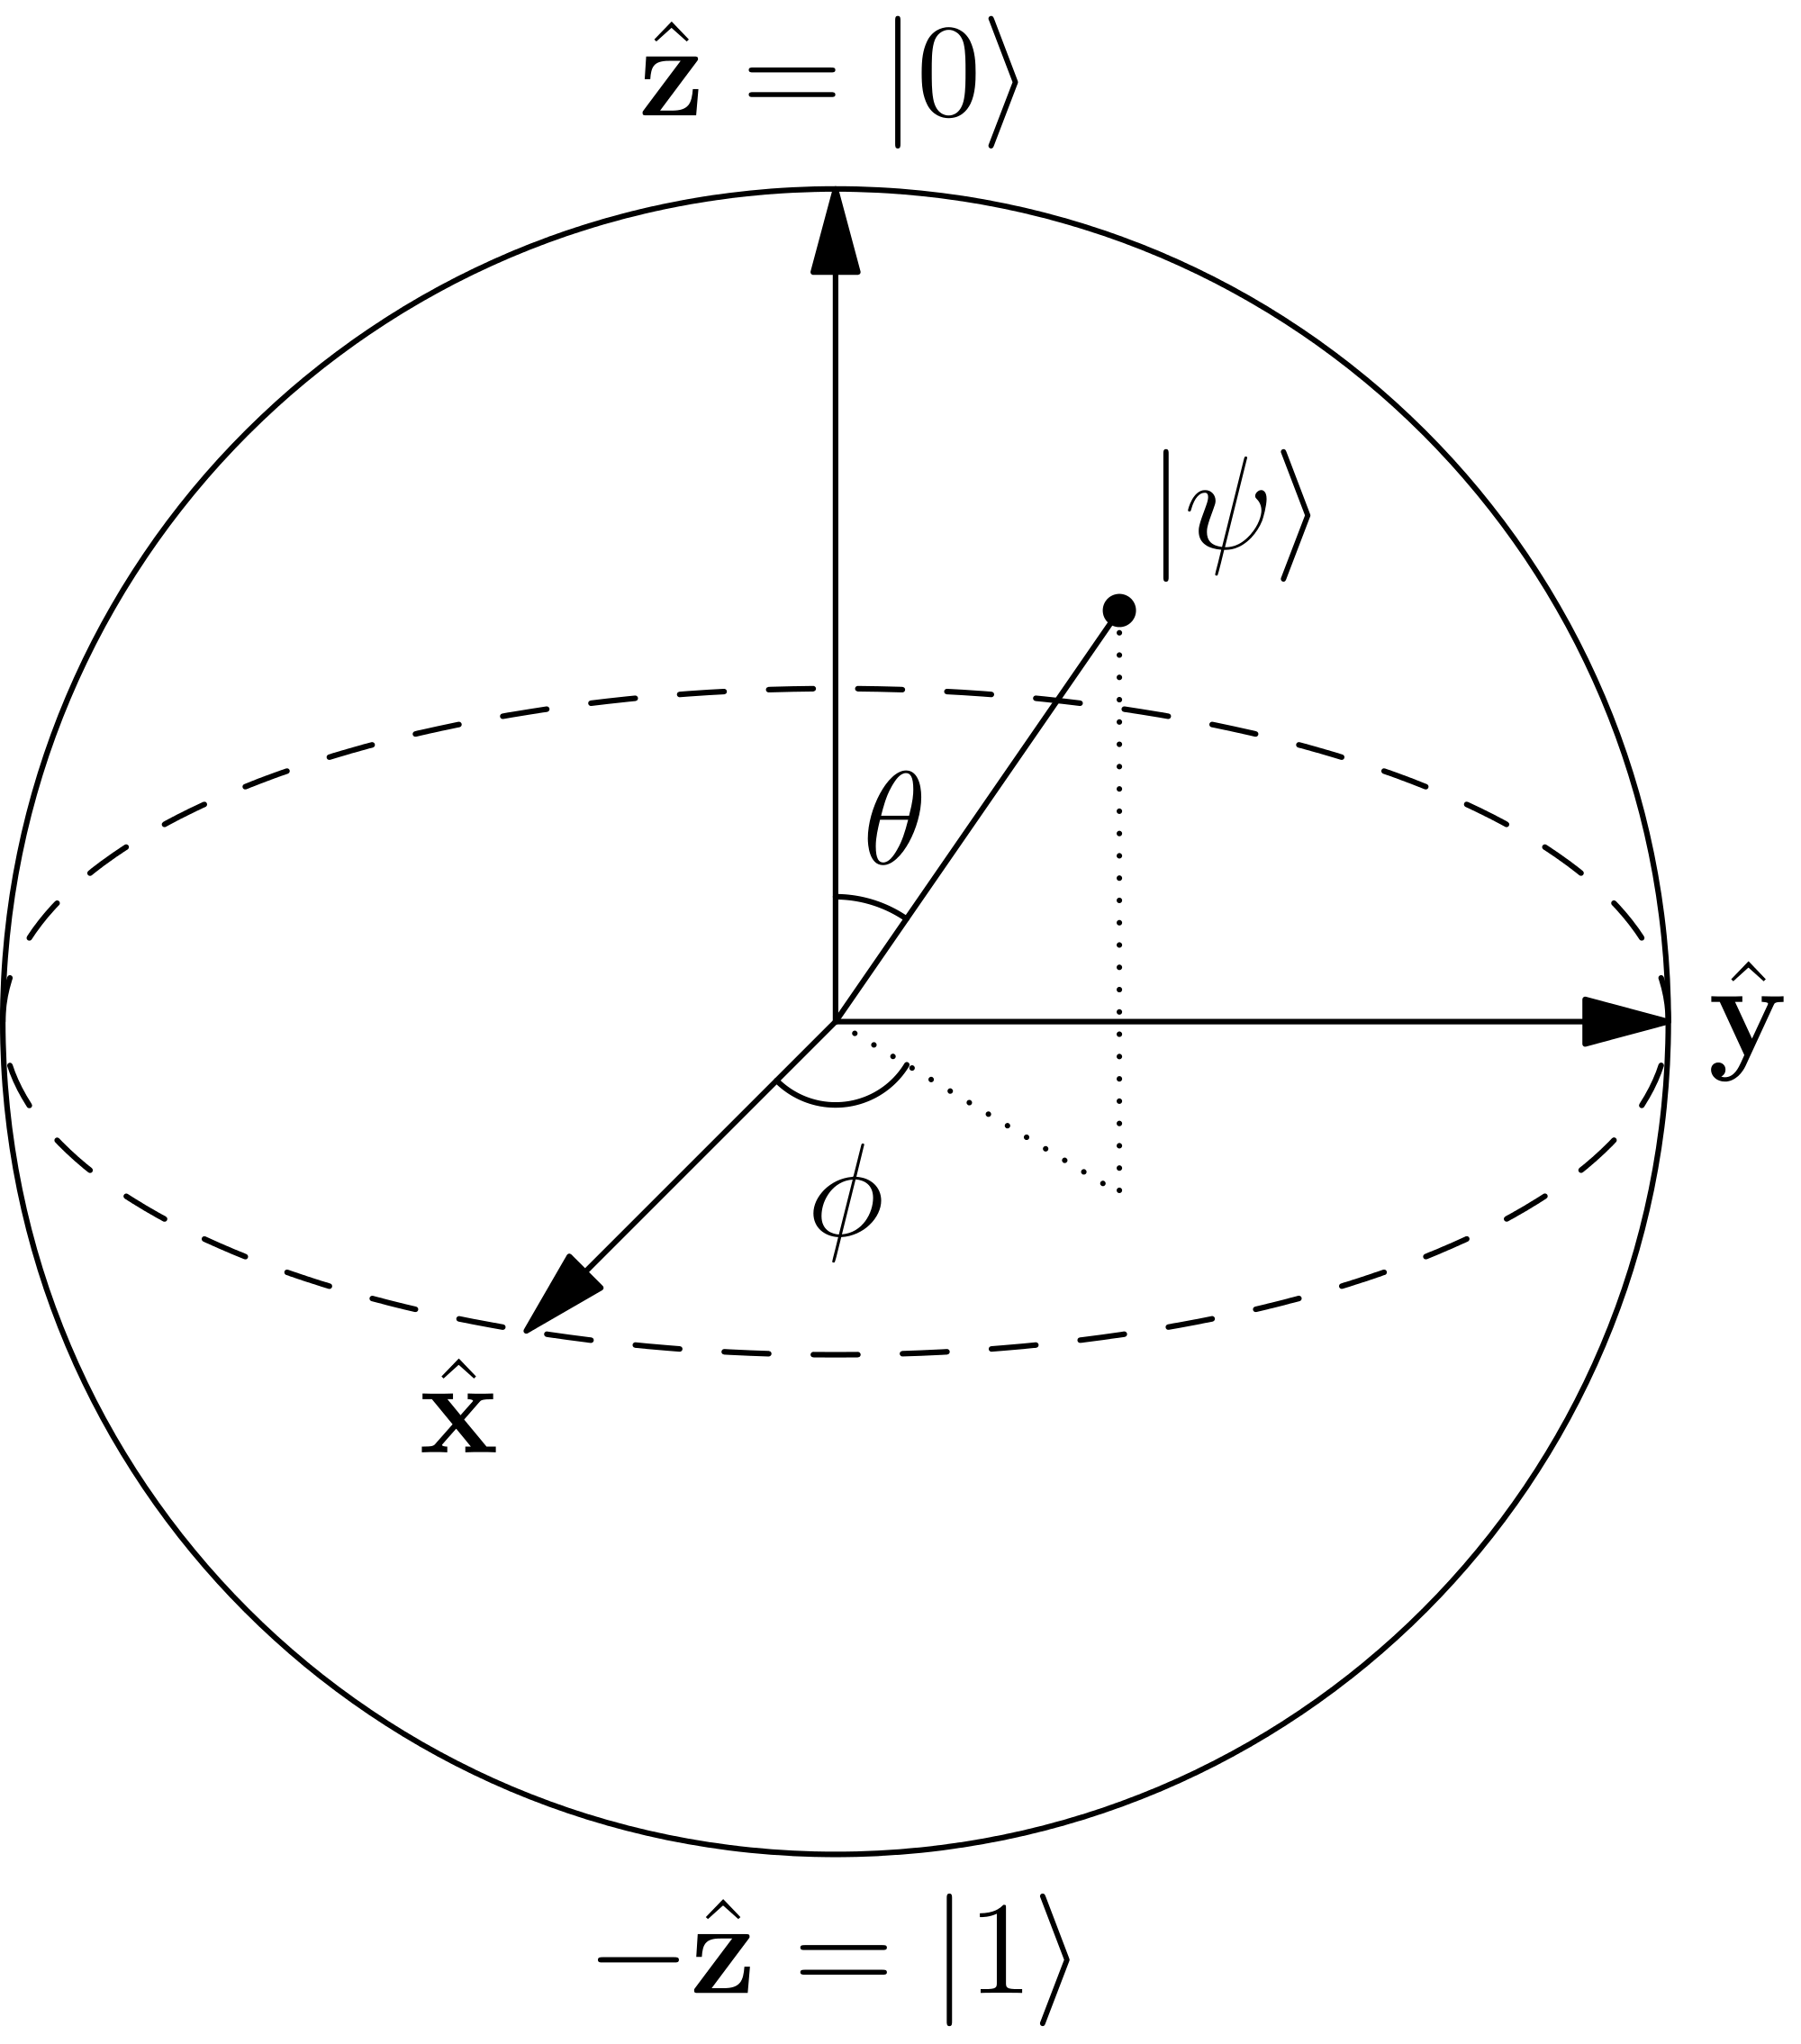
\includegraphics[scale=0.07]{img/blochsphere.png}
       \caption{\label{fig:blochsphere} An arbitrary two-dimensional qubit $\ket{\psi}$ visualized on the Bloch sphere.$^{2}$}
\end{figure}

\footnotetext[2]{Reprinted from Wikipedia, n.d., Retrieved September 7, 2016, from \url{https://en.wikipedia.org/wiki/Bloch_Sphere}. Copyright 2012 by Glosser.ca. Reprinted with permission.}

\subsection{Multiple Qubit Systems}
\label{subsec:multiplequbitsystems}

When moving from single to multi qubit systems a new mathematical tool, the so-called tensor product (symbol $\otimes$), is needed. A tensor product of two qubits is written as:

\begin{equation}
\ket{\psi} \otimes \ket{\psi} = \ket{0} \otimes \ket{0} = \ket{00}
\end{equation}
 
whereby the last expression omits the $\otimes$ symbol which is the shorthand form of a tensor product between two qubits.

In vector notation a tensor product of two vectors (\textcolor{red}{red} and \textcolor{green}{green}) is defined as shown below:

\begin{equation}
\label{equ:tensor2qubits}
\ket{\textcolor{red}{0}\textcolor{green}{0}} = \textcolor{red}{\ket{0}} \otimes \textcolor{green}{\ket{0}} = \textcolor{red}{\colvec{1\\0}} \otimes \textcolor{green}{\colvec{1\\0}} = \colvec{\textcolor{red}{1}*\textcolor{green}{\colvec{1\\0}}\\\textcolor{red}{0}*\textcolor{green}{\colvec{1\\0}}} = \colvec{1\\0\\0\\0}
\end{equation}

The last expression in Equ.~\ref{equ:tensor2qubits} shows that the two-qubit state $\ket{00}$ is no longer two but four-dimensional. Hence, it lives in a four-dimensional Hilbert space $\mathcal{H}_{4}$. A quantum gate acting on multiple qubits can therefore not have the same dimensions as a single-qubit gate (Equ.~\ref{equ:unitarytransformation}) which demands for a new gate formalism for multi qubit systems.

Consider wanting to apply an arbitrary single-qubit gate U (Equ.~\ref{equ:unitarytransformation}) to the first qubit and leaving the second qubit unchanged, essentially applying the identity matrix $\mathbb{1}$ to it. To do this, one defines the tensor product of two matrices as follows,

\begin{equation}
\label{equ:matrixtensorproduct}
\textcolor{red}{U} \otimes \textcolor{green}{\mathbb{1}} =\textcolor{red}{\begin{pmatrix}
 a & b \\ 
 c & d
 \end{pmatrix}} \otimes \textcolor{green}{\begin{pmatrix}
 1 & 0 \\ 
 0 & 1
 \end{pmatrix}} = \begin{pmatrix}
 \textcolor{red}{a}*\textcolor{green}{\begin{pmatrix}
 1 & 0 \\ 
 0 & 1
 \end{pmatrix}} & \textcolor{red}{b}*\textcolor{green}{\begin{pmatrix}
 1 & 0 \\ 
 0 & 1
 \end{pmatrix}} \\ 
 \textcolor{red}{c}*\textcolor{green}{\begin{pmatrix}
 1 & 0 \\ 
 0 & 1
 \end{pmatrix}} & \textcolor{red}{d}*\textcolor{green}{\begin{pmatrix}
 1 & 0 \\ 
 0 & 1
 \end{pmatrix}}
 \end{pmatrix} = \begin{pmatrix}
 a & 0 & b & 0 \\ 
 0 & a & 0 & b \\ 
 c & 0 & d & 0 \\ 
 0 & c & 0 & d 
 \end{pmatrix}
\end{equation}

Thus, the result of the tensor product $U \otimes \mathbb{1}$ is a unitary 4x4 matrix which can now be used to linearly transform the 4x1 vector representing the $\ket{00}$ state in Equ.~\ref{equ:tensor2qubits}:

\begin{equation}
\label{equ:2qubitlineartransform1}
U \otimes \mathbb{1} \ket{00} = \begin{pmatrix}
 a & 0 & b & 0 \\ 
 0 & a & 0 & b \\ 
 c & 0 & d & 0 \\ 
 0 & c & 0 & d 
 \end{pmatrix} \colvec{1\\0\\0\\0} = \colvec{a\\0\\c\\0}
\end{equation}

One can also first perform the single qubit operations on the respective qubits followed by the tensor product of the two resulting vectors:

\begin{equation}
\label{equ:2qubitlineartransform2}
(U \otimes \mathbb{1})(\ket{0} \otimes \ket{0})= U\ket{0} \otimes \mathbb{1}\ket{0} = \begin{pmatrix}
 a & b \\ 
 c & d
 \end{pmatrix} \colvec{1\\0} \otimes \begin{pmatrix}
 1 & 0 \\ 
 0 & 1
 \end{pmatrix} \colvec{1\\0} = \colvec{a\\c} \otimes \colvec{1\\0} = \colvec{a\\0\\c\\0}
\end{equation}

This formalism can be extended to any number of qubits and 

Introduce entanglement and non-factorising tensor states here!

%%%%% SECTION: Q LOGIC GATES


\section{Quantum Logic Gates}
\label{subsec:quantumlogicgates}
In order to perform quantum computations, tools, analogous to the classical logic gates, are needed for qubit manipulation. Quantum logic gates are square matrices that can be visualized as rotations on the Bloch sphere. The following subsections will introduce the major single and multi qubit logic gates.

\subsection{Single Qubit Gates}
\label{subsubsec:singlequbitgates} 

\subsubsection{Qubit Flip (X) Gate}
\label{subsubsubsec:xgate}

The quantum equivalent of the classical NOT logic gate is called X gate and is given by the 1\textsuperscript{st} Pauli matrix:

\begin{equation}
\sigma_{1} = X = \begin{pmatrix}
 0 & 1 \\ 
 1 & 0
 \end{pmatrix}
\end{equation}

The action of a quantum gate on a qubit state can be analysed using the gate's matrix and the qubit's vector representation. Applying some straightforward linear algebra yields:

\begin{equation}
\label{equ:xverification1}
X \otimes \ket{\psi} = X \otimes (\alpha \ket{0} + \beta \ket{1}) = \begin{pmatrix}
 0 & 1 \\ 
 1 & 0
 \end{pmatrix} \begin{pmatrix}
 \alpha  \\ 
 \beta
 \end{pmatrix} = \begin{pmatrix}
 \beta  \\ 
 \alpha
 \end{pmatrix} = \beta \ket{0} + \alpha \ket{1}
\end{equation}

Thus, applying the X gate to qubit state $\ket{\psi}$ swaps the amplitudes of \0 and \1. More specifically, applying X to the \0 state results in the \1 state,

\begin{equation}
\label{equ:xverification2}
X \otimes \ket{0} = \begin{pmatrix}
 0 & 1 \\ 
 1 & 0
 \end{pmatrix} \begin{pmatrix}
 1  \\ 
 0
 \end{pmatrix} = \begin{pmatrix}
 0  \\ 
 1 \end{pmatrix} =  \ket{1}
\end{equation}

In terms of the example with the electron of a hydrogen atom shown in Fig.~\ref{img:qubitatom} consider the qubit initially being in state \0. Applying an X gate will flip the qubit into the \1 state which can be implemented in the lab by exciting the electron into the next highest electron valence shell using a controlled laser pulse.

The \0 state is recovered when applying X again to the \1 state,

\begin{equation}
\label{equ:xverification3}
X \otimes \ket{1} = \begin{pmatrix}
 0 & 1 \\ 
 1 & 0
 \end{pmatrix} \begin{pmatrix}
 0  \\ 
 1
 \end{pmatrix} = \begin{pmatrix}
 1  \\ 
 0 \end{pmatrix} =  \ket{0}
\end{equation}

On the Bloch sphere, the X gate corresponds to a anti-clockwise $\pi$ rotation around the x-axis as shown in Fig.~\ref{img:blochxgate}.

\begin{figure}[ht]
   \centering
   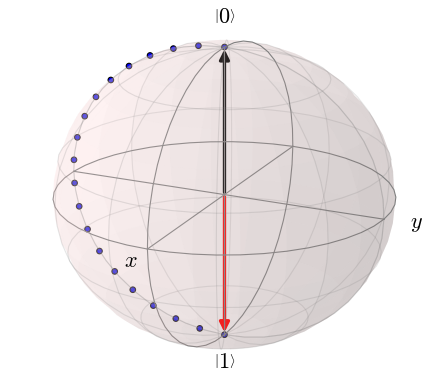
\includegraphics[width=0.5\textwidth]{img/blochxgate.png}
   \caption{Visualization of the X gate on the Bloch sphere. Initial state (black) transformed to final state (red).}
   \label{img:blochxgate}
\end{figure}

From Equ.~\ref{equ:xverification1},~\ref{equ:xverification2} and~\ref{equ:xverification3} it follows that X is its own inverse as well as its own Hermitian conjugate:
\begin{align}
XX &= XX^\dagger = \mathbb{1} \\
X &= X^{-1} = X^\dagger
\end{align}

The action, circuit \& matrix representation and Bloch sphere visualization for the most important single-qubit quantum logic gates are summarised in Table~\ref{tab:singlequbitgates}  below.

\begin{table}[H]
\caption{Table of major single-qubit quantum logic gates.}\vspace{1em}
\label{tab:singlequbitgates}
\begin{tabular}{ C{0.3cm}  C{2cm}  C{1.5cm}  C{1.5cm} C{2.5cm} C{2cm} C{3.5cm}}\hline
Gate & Name & Circuit representation & Matrix & Description & Rotation & Bloch sphere \\ \midrule
$\mathbb{1}$ & Identity & 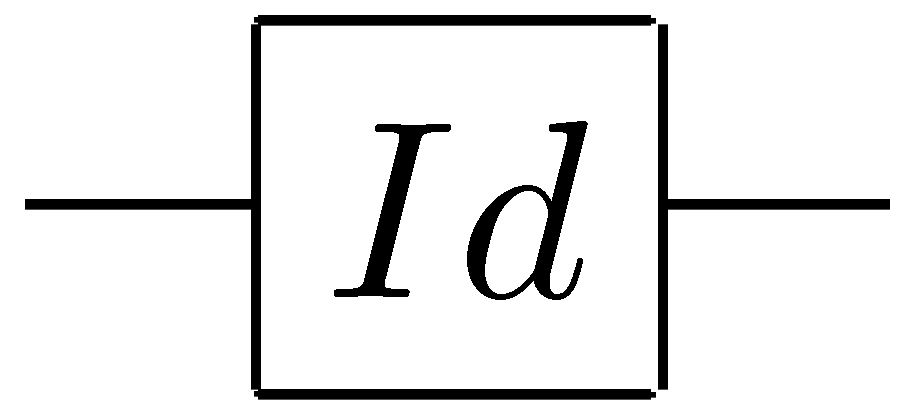
\includegraphics[width=0.1\textwidth]{img/identitycircuit.png} & $\begin{pmatrix}
 1 & 0 \\ 
 0 & 1
 \end{pmatrix}$ & Idle or waiting gate & - & - \\\midrule
X & Qubit flip & 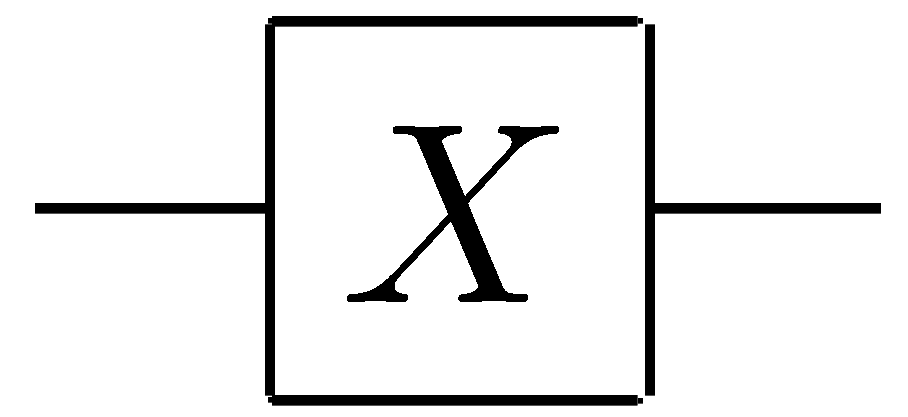
\includegraphics[width=0.1\textwidth]{img/xcircuit.png}  & $\begin{pmatrix}
 0 & 1 \\ 
 1 & 0
 \end{pmatrix}$ & Swaps amplitudes of \0 and \1 & $\pi$ rotation around $\hat{x}$ & 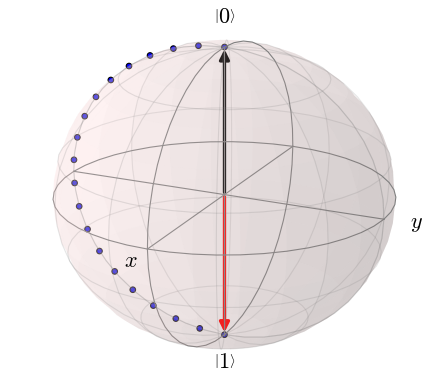
\includegraphics[width=0.2\textwidth]{img/blochxgate.png}\\\midrule
Y & Qubit \& phase flip & 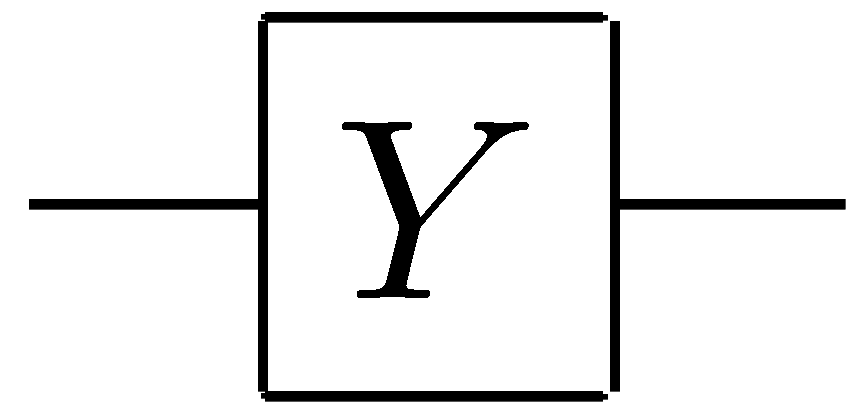
\includegraphics[width=0.1\textwidth]{img/ycircuit.png}  & $\begin{pmatrix}
 0 & -i \\ 
 i & 0
 \end{pmatrix}$ & Swaps amplitudes and introduces phase & $\pi$ rotation around $\hat{y}$ &  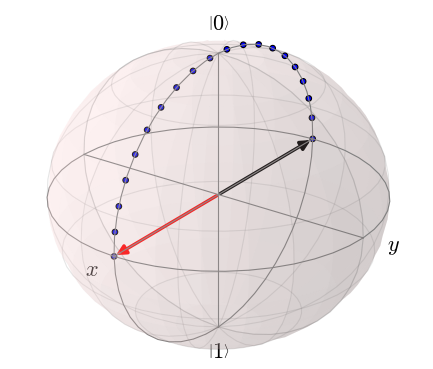
\includegraphics[width=0.2\textwidth]{img/blochygate.png}\\\midrule
Z & Phase flip & 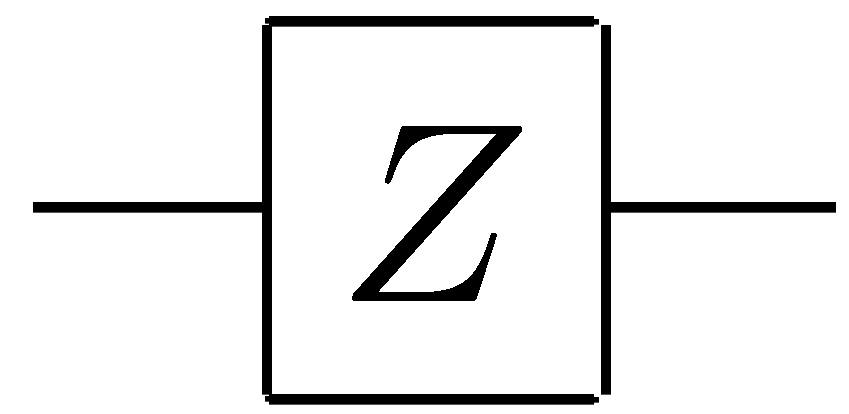
\includegraphics[width=0.1\textwidth]{img/zcircuit.png} & $\begin{pmatrix}
 1 & 0 \\ 
 0 & -1
 \end{pmatrix}$ & Adds a negative sign to the \1 state & $\pi$ rotation around $\hat{z}$ & 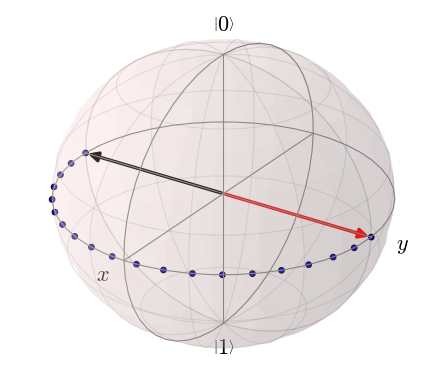
\includegraphics[width=0.2\textwidth]{img/blochzgate.png} \\\midrule 
H & Hadamard & 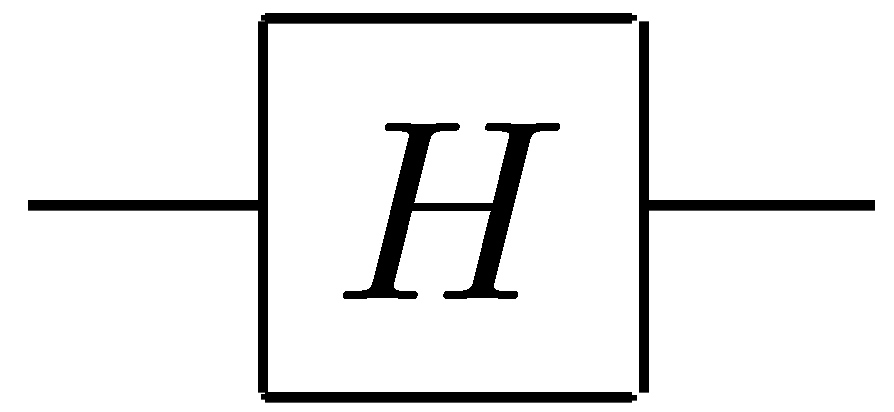
\includegraphics[width=0.1\textwidth]{img/hcircuit.png}  & $\begin{pmatrix}
 \frac{1}{\sqrt{2}} & \frac{1}{\sqrt{2}} \\ 
 \frac{1}{\sqrt{2}} & -\frac{1}{\sqrt{2}}
 \end{pmatrix}$ & Creates equal superpositions & $\frac{\pi}{2}$ rotation around $\hat{y}$ and $\pi$ rotation around $\hat{x}$ & 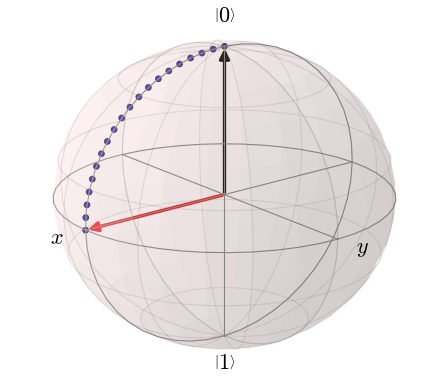
\includegraphics[width=0.2\textwidth]{img/blochhadamard.png}\\\midrule
S & $\frac{\pi}{2}$ rotation gate & 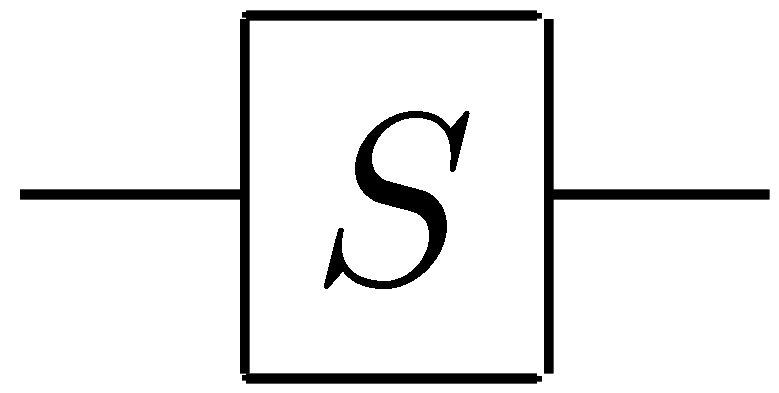
\includegraphics[width=0.1\textwidth]{img/scircuit.png} & $\begin{pmatrix}
 1 & 0 \\ 
 0 & i
 \end{pmatrix}$ & $\sqrt{Z}$ & $\frac{\pi}{2}$ rotation around $\hat{z}$ &  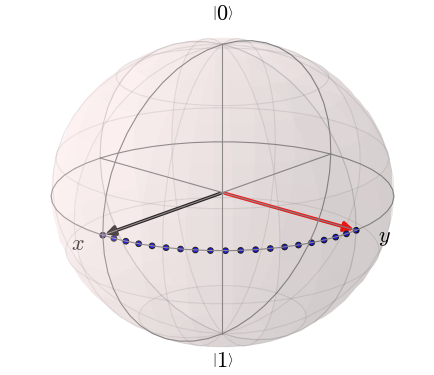
\includegraphics[width=0.2\textwidth]{img/blochsgate.png}\\\midrule
S$^\dagger$ & $-\frac{\pi}{2}$ rotation gate & 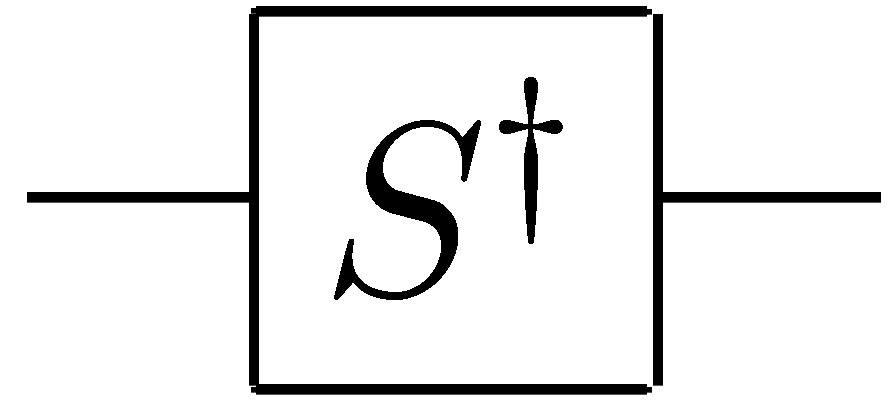
\includegraphics[width=0.1\textwidth]{img/sdcircuit.png} &  $\begin{pmatrix}
 1 & 0 \\ 
 0 & -i
 \end{pmatrix}$ & Adjoint of S & $-\frac{\pi}{2}$ rotation around $\hat{z}$ & \\\midrule
T & $\frac{\pi}{4}$ rotation gate & 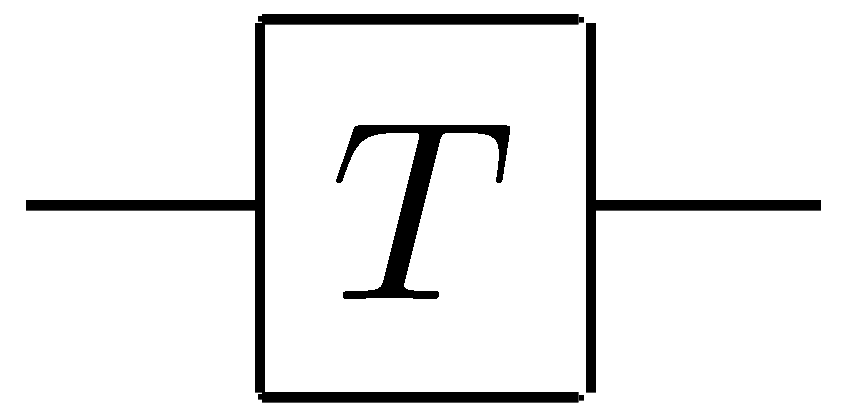
\includegraphics[width=0.1\textwidth]{img/tcircuit.png} & $\begin{pmatrix}
 1 & 0 \\ 
 0 & e^{\frac{i\pi}{4}}
 \end{pmatrix}$ & $\sqrt{S}$ & $\frac{\pi}{4}$ rotation around $\hat{z}$ & 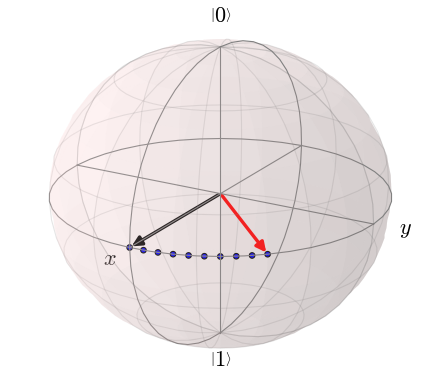
\includegraphics[width=0.2\textwidth]{img/blochtgate.png}\\\midrule
T$^\dagger$ & $-\frac{\pi}{4}$ rotation gate & 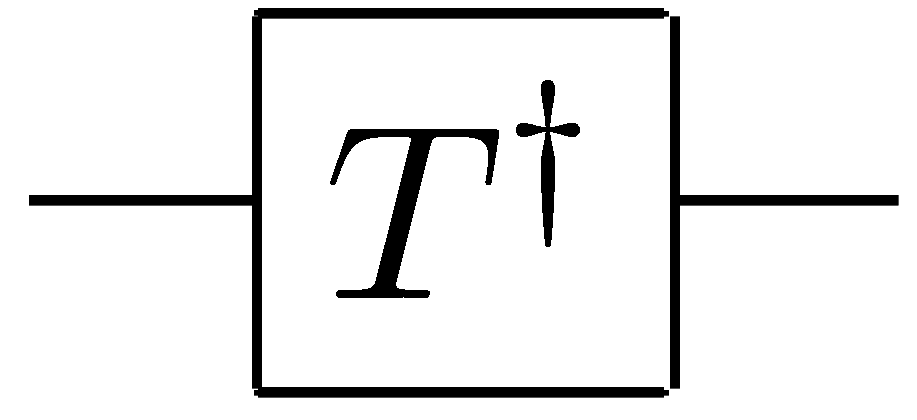
\includegraphics[width=0.1\textwidth]{img/tdcircuit.png} & $\begin{pmatrix}
 1 & 0 \\ 
 0 & e^{-\frac{i\pi}{4}}
 \end{pmatrix}$ & Adjoint of T & $-\frac{\pi}{4}$ rotation around $\hat{z}$ & \\\midrule
ZM & Z-basis measurement & 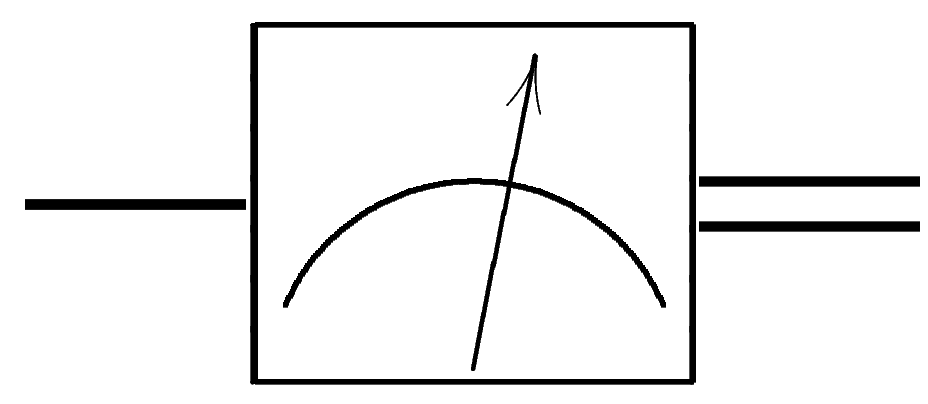
\includegraphics[width=0.1\textwidth]{img/measurecircuit.png} & - & Measurement in standard basis & Collapses the state & - \\
%\midrule
%BM & Bloch measurement & 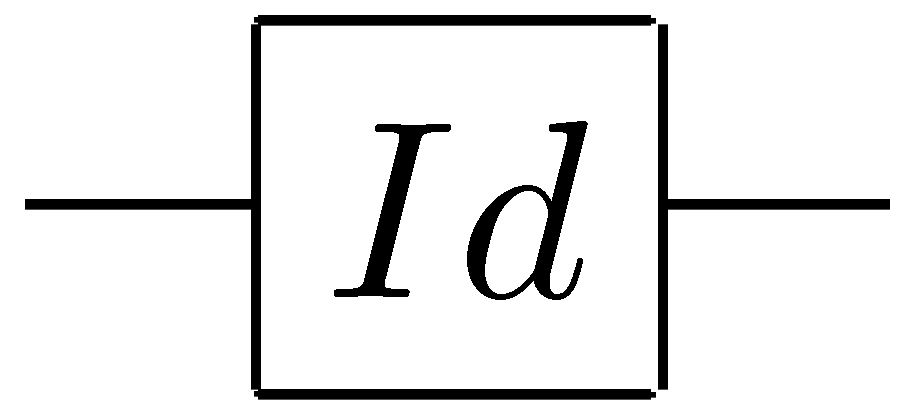
\includegraphics[width=0.1\textwidth]{img/identitycircuit.png} & - & Quantum state tomography & Collapses the state  & -\\
\end{tabular}
\end{table}


%%%%% SUBSECTION: MULTIPLE Q LOGIC GATES


\subsection{Multiple Qubit Gates}
\label{subsubsec:multiqubitgates}

\subsubsection{Controlled NOT Gate}
\label{subsubsubsec:cnotgate}

The most important two-qubit quantum gate is the controlled NOT or CNOT gate given by the following 4x4 matrix:
\begin{equation}
CNOT = \begin{pmatrix}
 \mathbb{1} & 0 \\ 
 0 & X
 \end{pmatrix} = \begin{pmatrix}
 1 & 0 & 0 & 0 \\ 
 0 & 1 & 0 & 0 \\
 0 & 0 & 0 & 1 \\
 0 & 0 & 1 & 0 \\
 \end{pmatrix}
\end{equation}

The CNOT gate takes two qubits, control and target qubit, as input. If and only if the control qubit is in the \1 state, the NOT (X) gate is applied to the target qubit. In equations, the CNOT will always be followed by parantheses containing the control qubit followed by the target qubit (e.g. CNOT(0,1)). The input-output relation for the CNOT gate is given in the truth table~\ref{tab:cnottruthtable} below.

\begin{table}[H]
\begin{center}
\caption{CNOT truth table with first qubit as control, second qubit as target.}\vspace{1ex}
\label{tab:cnottruthtable}
\begin{tabular}{llccc}\hline
Input & Output \\ \hline
00 & 00 \\
01 & 01 \\
10 & 11 \\
11 & 10 \\ \hline
\end{tabular}
\end{center}
\end{table}

To demonstrate the usefulness of the CNOT gate consider starting with two unentangled qubits both in the \0 state,

\begin{equation}
\ket{\phi} = \ket{0} \otimes \ket{0} = \ket{00}
\end{equation}

Applying the H gate onto the first qubit yields the following (still unentangled) state:

\begin{equation}
(H \otimes \mathbb{1}) \ket{\phi} = (H \otimes \mathbb{1}) \ket{00} = \frac{1}{\sqrt{2}} \ket{00} + \frac{1}{\sqrt{2}} \ket{10} 
\end{equation}

Now consider applying the CNOT to this state whereby the control qubit is coloured \textcolor{red}{red} and the target qubit \textcolor{green}{green}.

\begin{equation}
\label{equ:cnotexamples}
CNOT(\textcolor{red}{0},\textcolor{green}{1}) \otimes (\frac{1}{\sqrt{2}} \ket{\textcolor{red}{0}\textcolor{green}{0}} + \frac{1}{\sqrt{2}} \ket{\textcolor{red}{1}\textcolor{green}{0}}) = \frac{1}{\sqrt{2}} \ket{\textcolor{red}{0}\textcolor{green}{0}} + \frac{1}{\sqrt{2}} (\mathbb{1} \otimes X) \ket{\textcolor{red}{1}\textcolor{green}{0}} = \frac{1}{\sqrt{2}} \ket{\textcolor{red}{0}\textcolor{green}{0}} + \frac{1}{\sqrt{2}} \ket{\textcolor{red}{1}\textcolor{green}{1}}
\end{equation}

The last expression in Equ.~\ref{equ:cnotexamples} is one of the famous Bell states which are four maximally entangled states. Thus, this example demonstrates how the CNOT gate is crucial for the generation of entangled states since it applies the X gate to a qubit depending on the state of a second qubit.

The three most important multi qubit quantum gates CNOT, Toffoli and nCNOT are characterised in Table~\ref{tab:multiqubitgates}.

\begin{table}[H]
\caption{Table of major multi-qubit quantum logic gates where $c_j$ stands for the j\textsuperscript{th} control and $\mathbb{1}_k$ for the kxk identity matrix.}\vspace{1em}
\label{tab:multiqubitgates}
\begin{tabular}{ c  C{1.8cm}  C{2cm}  c C{3cm}}\hline
Gate & Name & Circuit representation & Matrix & Description \\ \midrule
CNOT & Controlled NOT & 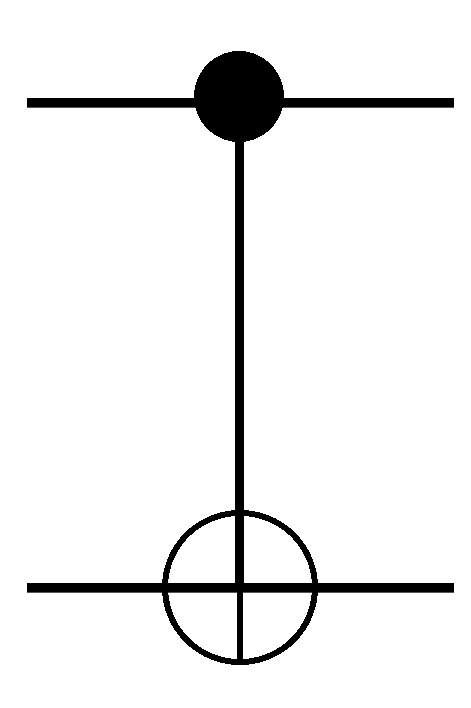
\includegraphics[width=0.1\textwidth]{img/cnotcircuit.png} & $\begin{pmatrix}
 \mathbb{1} & 0 \\ 
 0 & X
 \end{pmatrix} = \begin{pmatrix}
 1 & 0 & 0 & 0 \\ 
 0 & 1 & 0 & 0 \\
 0 & 0 & 0 & 1 \\
 0 & 0 & 1 & 0 \\
 \end{pmatrix}$ & CNOT($c_1$, target) \\\midrule
Toffoli & Controlled controlled NOT & 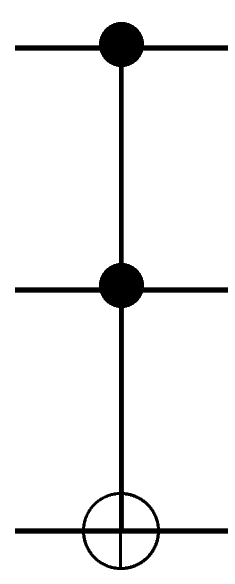
\includegraphics[width=0.1\textwidth]{img/ccnotcircuit.png}  & $\begin{pmatrix}
 \mathbb{1}_6 & 0 \\ 
 0 & X
 \end{pmatrix} = \begin{pmatrix}
 1 & 0 & 0 & 0 & 0 & 0 & 0 & 0 \\ 
 0 & 1 & 0 & 0 & 0 & 0 & 0 & 0 \\ 
 0 & 0 & 1 & 0 & 0 & 0 & 0 & 0 \\ 
 0 & 0 & 0 & 1 & 0 & 0 & 0 & 0 \\ 
 0 & 0 & 0 & 0 & 1 & 0 & 0 & 0 \\ 
 0 & 0 & 0 & 0 & 0 & 1 & 0 & 0 \\
 0 & 0 & 0 & 0 & 0 & 0 & 0 & 1 \\ 
 0 & 0 & 0 & 0 & 0 & 0 & 1 & 0 \\ 
 \end{pmatrix}$ & CCNOT($c_1$, $c_2$, target)\\\midrule
nCNOT & n-controlled NOT & -  & $\begin{pmatrix}
 \mathbb{1}_{2^n-2} & 0 \\ 
 0 & X
 \end{pmatrix}$ & nCNOT($c_1$,..,$c_n$, target) \\\midrule

\end{tabular}
\end{table}

%%%%% SECTION: MACHINE LEARNING

\section{Classical Machine Learning}
\label{subsec:classicalmachinelearning}

Introduce the three different types of ML!



\subsection{k-nearest Neighbour Algorithm}
\label{subsubsec:knearestneighbour}

In this thesis a quantum version of the distance weighted $k$-nearest neighbour (kNN) algorithm as described in \cite{Schuld2014} will be implemented. Understanding the QML algorithm requires knowledge of the classical version of the distance weighted kNN algorithm which will be introduced in this subsection.

\begin{figure}[ht]
  \begin{minipage}[t]{0.48\textwidth}
    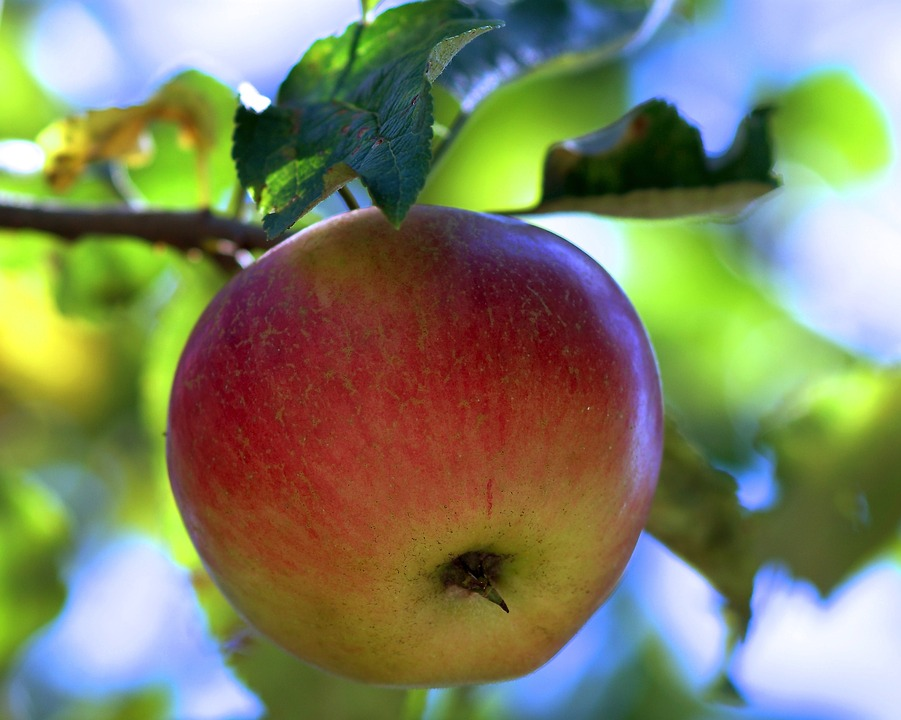
\includegraphics[width = \textwidth]{img/apple.jpg}
  \end{minipage}
  \hfill
  \begin{minipage}[t]{0.48\textwidth}
    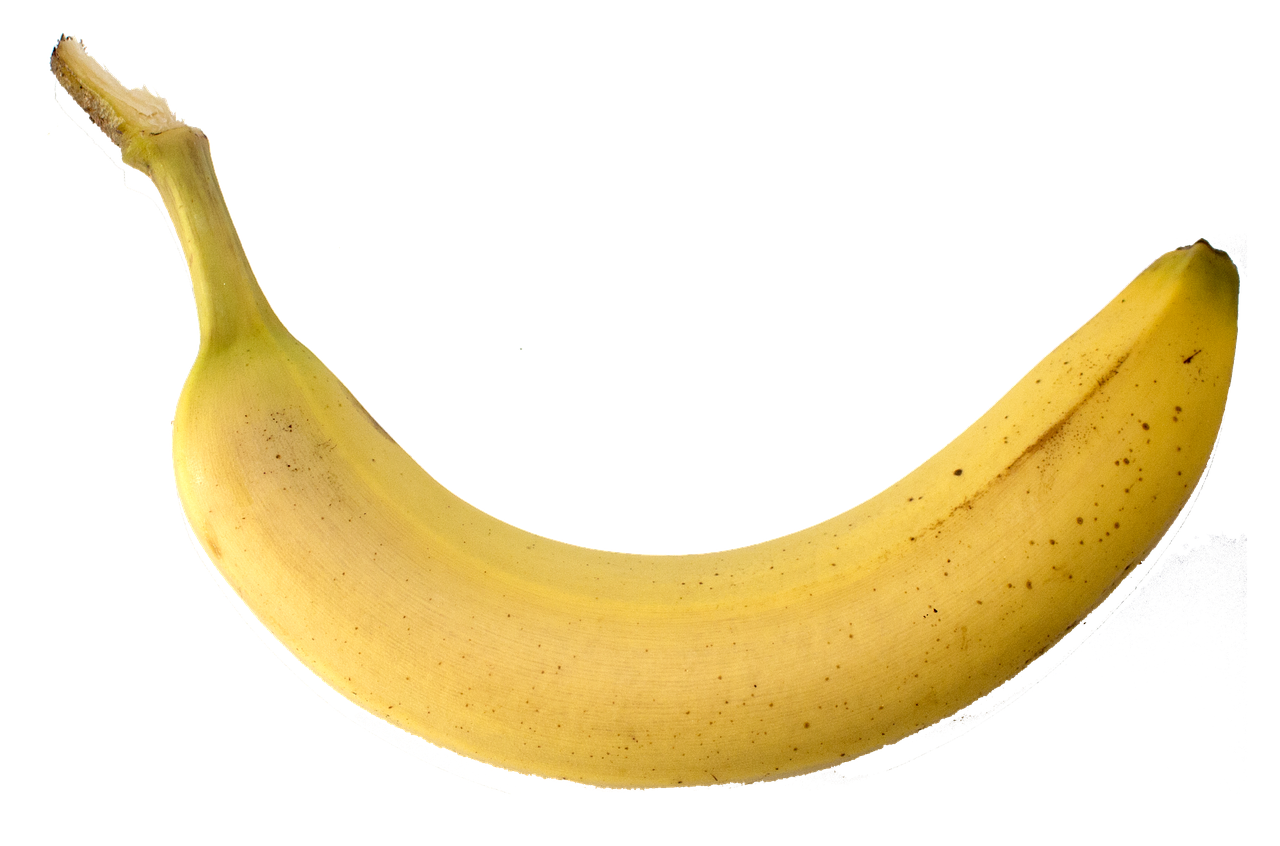
\includegraphics[width = \textwidth]{img/banana.png}
  \end{minipage}
  \caption{Pictures of apple and banana from training data set.}
  \label{img:appleandbanana}
\end{figure}

Imagine working for a search engine company and you are given the task of classifying unknown pictures of fruits as either apples or bananas. To train your classification algorithm you are given 5 pictures of apples and 5 pictures of bananas - this will be called the training data set ${D}_{T}$. Mathematically, the training data set ${D}_{T}$ consists of ten vectors ${v}_{0}, {v}_{1},..,{v}_{10}$ that are each assigned to either class $A$ (apple) or $B$ (banana). The training vectors are visualized as yellow and purple circles in Fig.~\ref{fig:knnconcept}.

kNN is a non-parametric classifier that given a new unclassified input vector $x$ (red star in Fig.~\ref{fig:knnconcept}) considers the $k$ nearest neighbours (using a predefined measure of distance) and classifies $x$, based on a majority vote, as either $A$ or $B$. Thereby, $k$ is a positive integer, usually chosen to be small and its value determines the classification outcome. Namely, in the case $k = 3$ in Fig.~\ref{fig:knnconcept}, vector $x$ will be classified as class B (purple) but in the case $k = 6$ it will be labelled class A (yellow).

\begin{figure}[!ht]
      \centering
       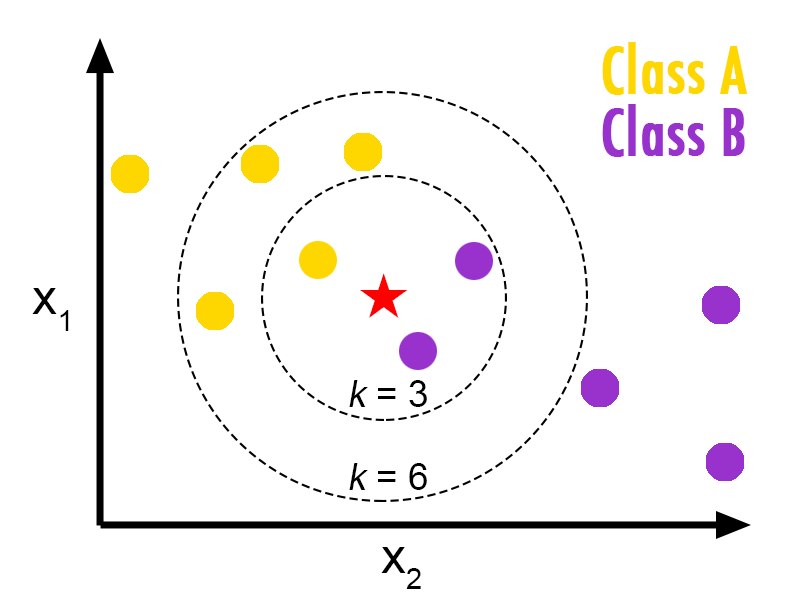
\includegraphics[scale=0.55]{img/knn-concept.png}
       \caption[caption for kNN]{\label{fig:knnconcept} Visualization of a kNN classifier\footnotemark[3]}
\end{figure}

\footnotetext[3]{Reprinted from GitHub, Burton de Wilde, Retrieved September 13, 2016, from \url{http://bdewilde.github.io/blog/blogger/2012/10/26/classification-of-hand-written-digits-3/}. Copyright 2012 by Burton de Wilde. Reprinted with permission.}

In the case of $k = 10$, $x$ would simply be assigned to the class with the most members. In this case, the training vectors should be given distance-dependent weights (such as $\frac{1}{distance}$) to increase the influence of closer vectors over more distant ones.

\section{Methods (own chapter?)}
\label{subsec:methods}

\subsection{Programming environment}
\label{subsubsec:programming}

Python
Liquid

\subsection{IBMs QC}
\label{subsubsec:ibmqc}

IBM QASM